\documentclass[usenames,dvipsnames,tikz]{standalone}
\usepackage{xcolor}
\colorlet{tBlue}{RoyalBlue!35!Cerulean}
\colorlet{tRed}{Red}
\usepackage{tikz}
\usepackage{standalone}
\begin{document}
	
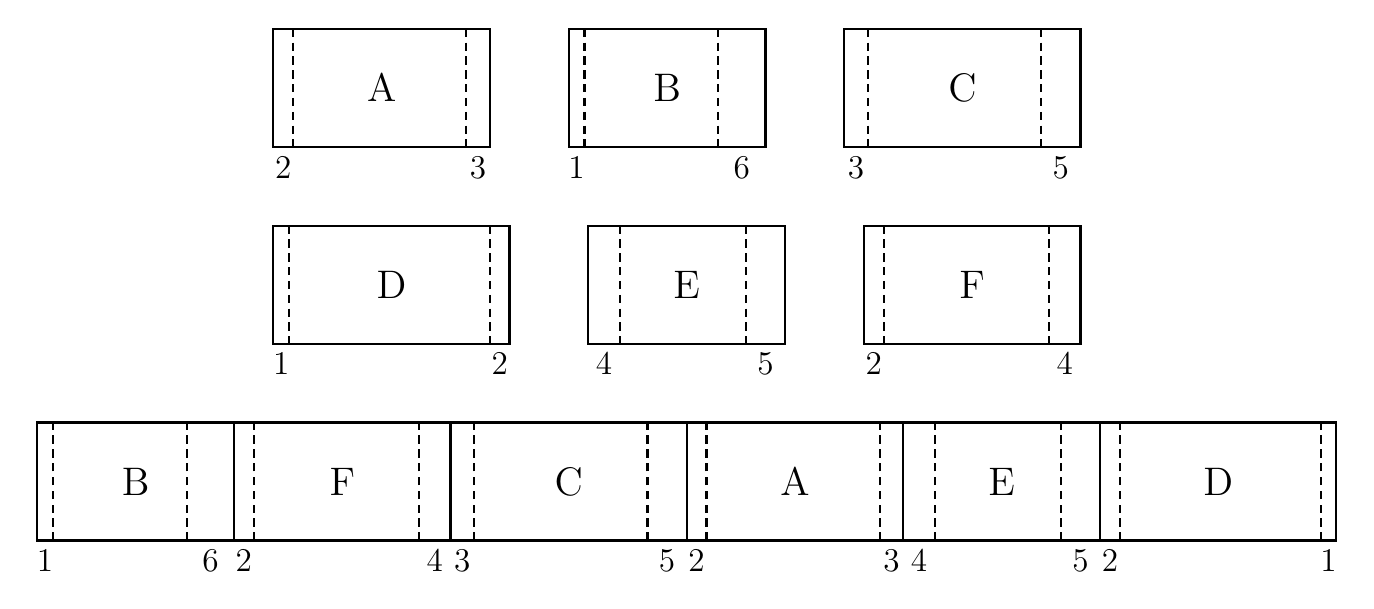
\begin{tikzpicture}
%\draw [help lines] (-1,-2) grid (17.5,8);

\draw [thick] (3,6.5) rectangle (5.75,5); % A (2,3)
\draw [thick, densely dashed] (3.25,6.5) -- (3.25,5);
\draw [thick, densely dashed] (5.45,6.5) -- (5.45,5);
\node [below] at (3.125, 5) {\large{2}};
\node [below] at (5.6, 5) {\large{3}};
\node at (4.375,5.75) {\Large{A}};

\draw [thick] (6.75,6.5) rectangle (9.25,5); % B (1,6)
\draw [thick, densely dashed] (6.95,6.5) -- (6.95,5);
\draw [thick, densely dashed] (8.65,6.5) -- (8.65,5);
\node [below] at (6.85, 5) {\large{1}};
\node [below] at (8.95, 5) {\large{6}};
\node at (8,5.75) {\Large{B}};

\draw [thick] (10.25,6.5) rectangle (13.25,5); % C (3,5)
\draw [thick, densely dashed] (10.55,6.5) -- (10.55,5);
\draw [thick, densely dashed] (12.75,6.5) -- (12.75,5);
\node [below] at (10.4, 5) {\large{3}};
\node [below] at (13, 5) {\large{5}};
\node at (11.75,5.75) {\Large{C}};

\draw [thick] (3,4) rectangle (6,2.5); % D (1,2)
\draw [thick, densely dashed] (3.2,4) -- (3.2,2.5);
\draw [thick, densely dashed] (5.75,4) -- (5.75,2.5);
\node [below] at (3.1, 02.5) {\large{1}};
\node [below] at (5.875, 2.5) {\large{2}};
\node at (4.5,3.25) {\Large{D}};

\draw [thick] (7,4) rectangle (9.5,2.5); % E (4,5)
\draw [thick, densely dashed] (7.4,4) -- (7.4,2.5);
\draw [thick, densely dashed] (9,4) -- (9,2.5);
\node [below] at (7.2, 2.5) {\large{4}};
\node [below] at (9.25, 2.5) {\large{5}};
\node at (8.25,3.25) {\Large{E}};

\draw [thick] (10.5,2.5) rectangle (13.25,4); % F (2,4)
\draw [thick, densely dashed] (10.75,4) -- (10.75,2.5);
\draw [thick, densely dashed] (12.85,4) -- (12.85,2.5);
\node [below] at (10.625, 2.5) {\large{2}};
\node [below] at (13.05, 2.5) {\large{4}};
\node at (11.875,3.25) {\Large{F}};

%----------------------------------------------

\draw [thick] (0,0) rectangle (16.5,1.5); %whole rectangle
\draw [thick] (2.5,0) -- (2.5, 1.5); % between B and F
\draw [thick] (5.25,0) -- (5.25, 1.5); % between F and C
\draw [thick] (8.25,0) -- (8.25, 1.5); % between C and A
\draw [thick] (11,0) -- (11, 1.5); % between A and E
\draw [thick] (13.5,0) -- (13.5, 1.5); % between E and D

\draw [thick, densely dashed] (0.2,0) -- (0.2, 1.5);
\draw [thick, densely dashed] (1.9,0) -- (1.9, 1.5);
\draw [thick, densely dashed] (2.75,0) -- (2.75, 1.5);
\draw [thick, densely dashed] (4.85,0) -- (4.85, 1.5);
\draw [thick, densely dashed] (5.55,0) -- (5.55, 1.5);
\draw [thick, densely dashed] (7.75,0) -- (7.75, 1.5);
\draw [thick, densely dashed] (8.5,0) -- (8.5, 1.5);
\draw [thick, densely dashed] (10.7,0) -- (10.7, 1.5);
\draw [thick, densely dashed] (11.4,0) -- (11.4, 1.5);
\draw [thick, densely dashed] (13,0) -- (13, 1.5);
\draw [thick, densely dashed] (13.75,0) -- (13.75, 1.5);
\draw [thick, densely dashed] (16.3,0) -- (16.3, 1.5);

\node [below] at (0.1, 0) {\large{1}};
\node [below] at (2.2, 0) {\large{6}};
\node [below] at (2.625, 0) {\large{2}};
\node [below] at (5.05, 0) {\large{4}};
\node [below] at (5.4, 0) {\large{3}};
\node [below] at (8, 0) {\large{5}};
\node [below] at (8.375, 0) {\large{2}};
\node [below] at (10.85, 0) {\large{3}};
\node [below] at (11.2, 0) {\large{4}};
\node [below] at (13.25, 0) {\large{5}};
\node [below] at (13.625, 0) {\large{2}};
\node [below] at (16.4, 0) {\large{1}};

\node at (1.25,0.75) {\Large{B}};
\node at (3.875,0.75) {\Large{F}};
\node at (6.75,0.75) {\Large{C}};
\node at (9.625,0.75) {\Large{A}};
\node at (12.25,0.75) {\Large{E}};
\node at (15,0.75) {\Large{D}};

\end{tikzpicture}
\end{document}